\section{Reducing the Model to One Half}

\Citeauthor{akyuz2022} pointed out in their master thesis, that the model satisfies the property in \Cref{equ:yunus.property.symmetry}.
This means, that there is some symmetry in the model.
In the following, I will reduce the model to only $\theta \mapsto F(\theta) \mod \pi$ and observe what happens in the thin area explored above.
\begin{align}
    F(\theta + \pi) & = F(\theta) + \pi \label{equ:yunus.property.symmetry}
\end{align}

Now, something interesting happens.
\Cref{fig:yunus.pi.2d.full} shows a 2D-scan of the same area that is depicted in \Cref{fig:yunus.2pi.2d.full}.
You can see that the thin areas now have a different color from the bigger areas.
This means that the period of the cycle or cycles in that area now have a higher period.

\begin{figure}
    \centering
    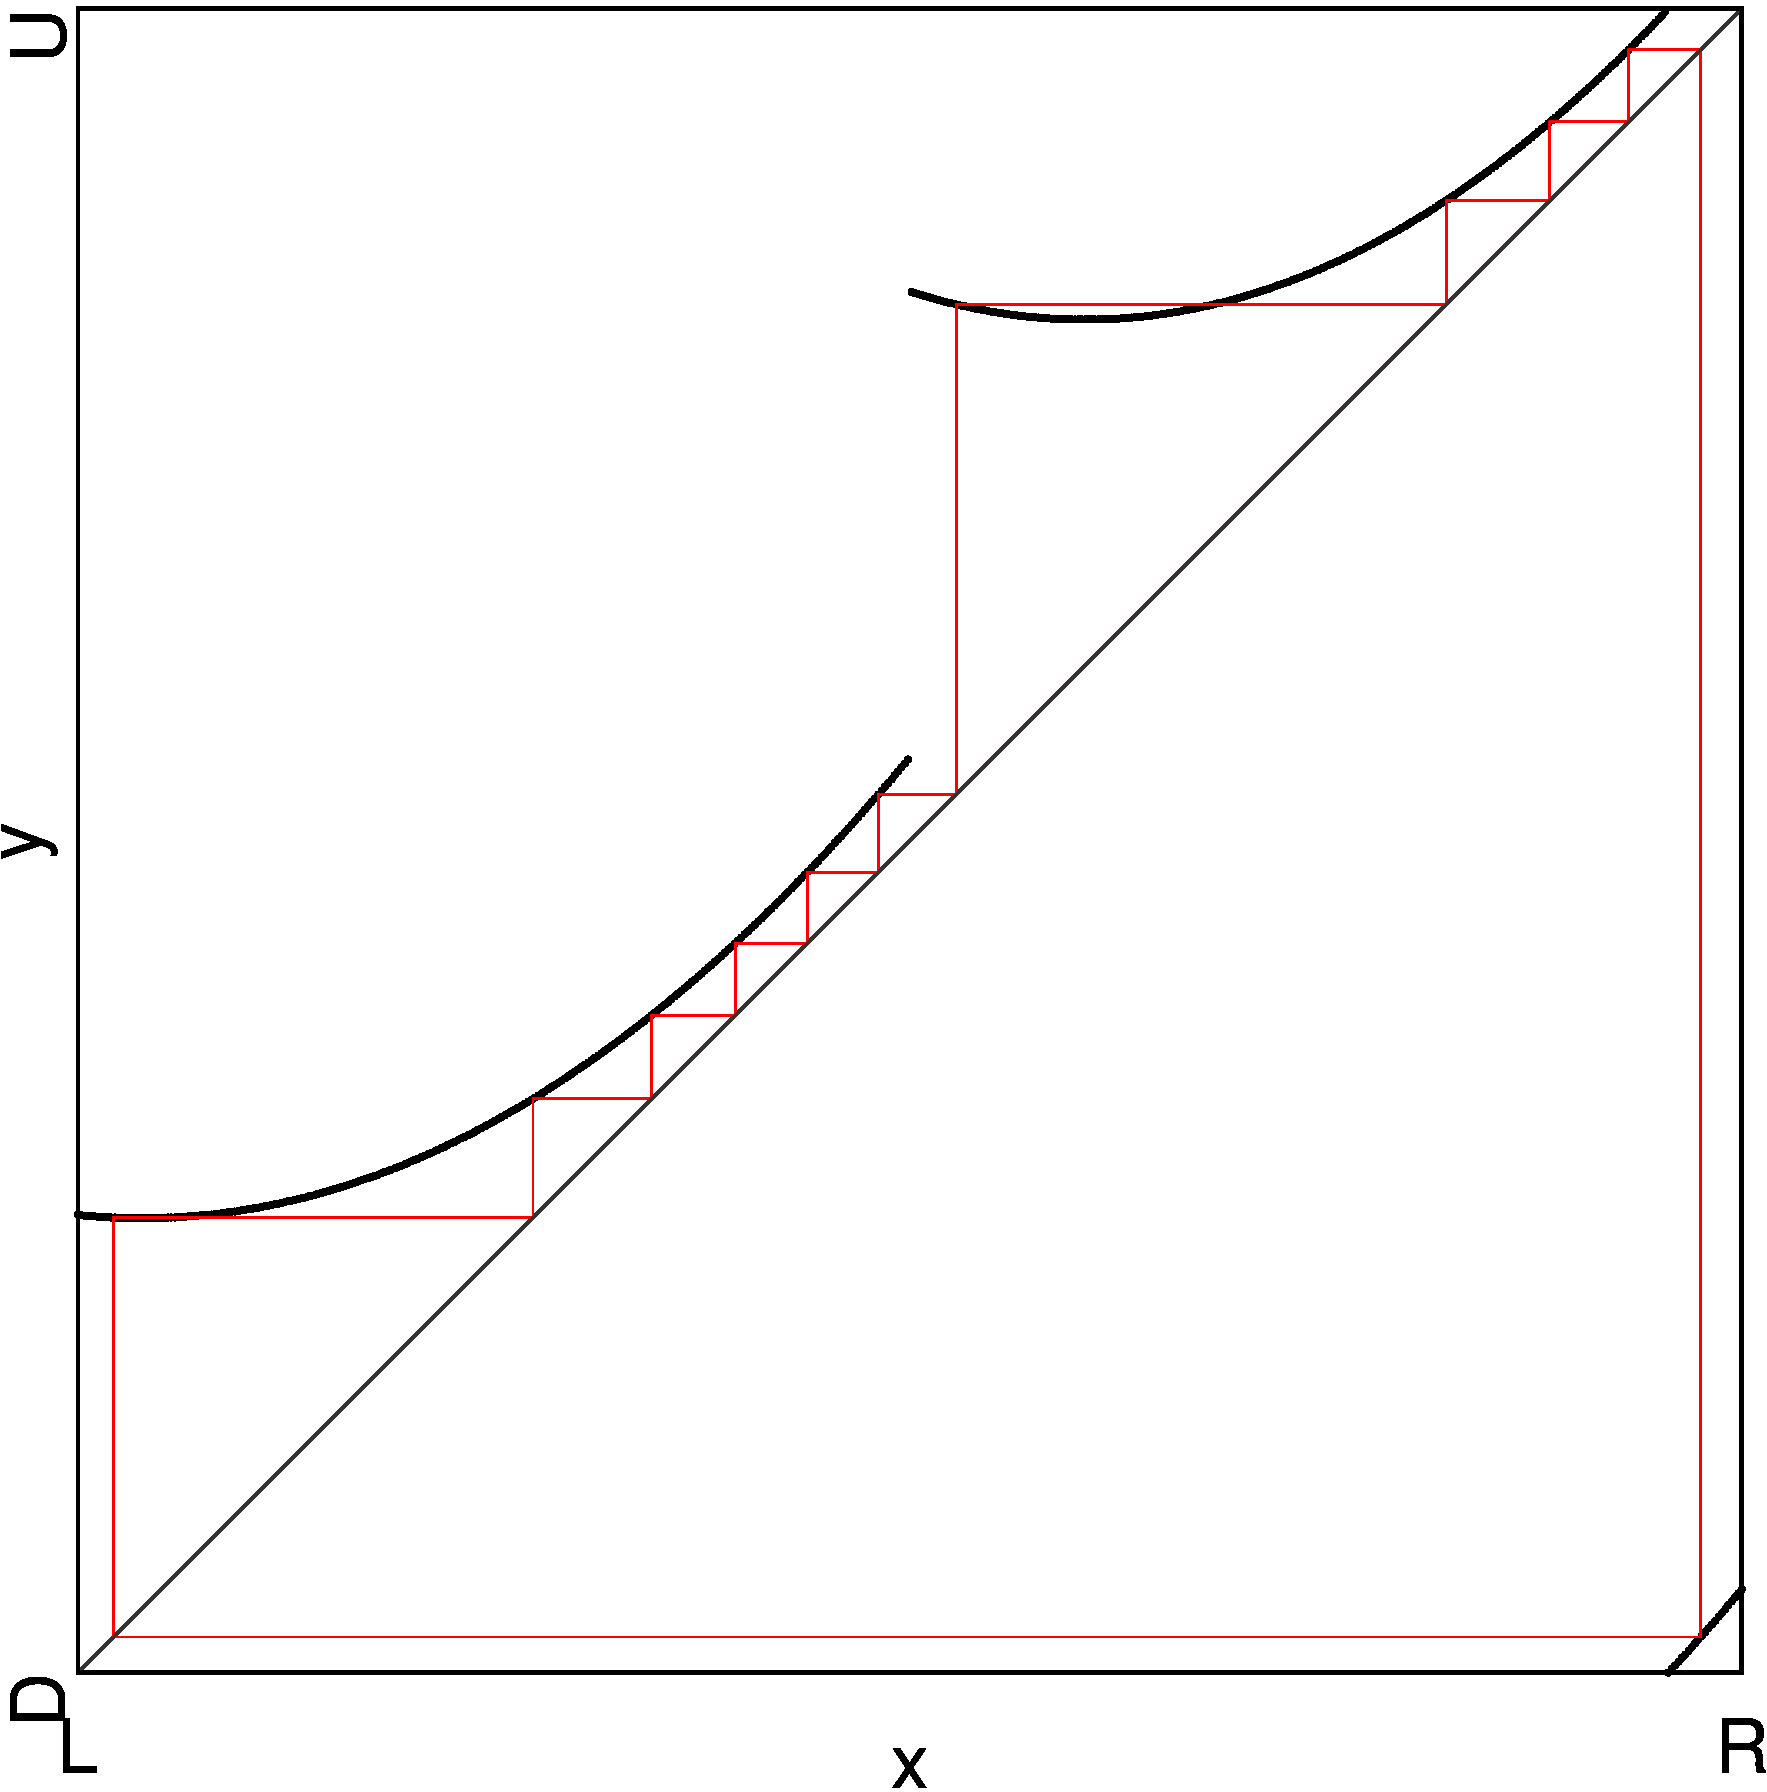
\includegraphics[width=0.6\textwidth]{98_Yunus_modpi/2D_Period/result.png}
    \caption{2D Scan of Original Model}
    \label{fig:yunus.pi.2d.full}
\end{figure}
